\chapter{Method}
\label[chapter]{chapter:method}

This chapter outlines the method of the reprojection and optimization pipeline. Following an overview of all components in \cref{sec:method_overview}, the process of each component is described in detail. Implementation details will be covered in the next chapter.

\section{Overview}
\label[section]{sec:method_overview}

\Cref{fig:method_overview} shows an overview of the four main components: railway processing, track detection, track reprojection, and pose optimization, as well as the global inputs and outputs, color-coded by the type of data. The global map data (green) includes \textit{railway network} and \textit{elevation data}, the frame-specific data (red) includes \textit{image} and \textit{GPS pose}, and the camera-specific data (blue) includes \textit{camera intrinsics} and \textit{camera pose}. All of these are inputs to the pipeline, and the output that is iterated over is the \textit{camera pose}. The processes in each component are described in the following sections.

\begin{figure}[h]
    \centering
    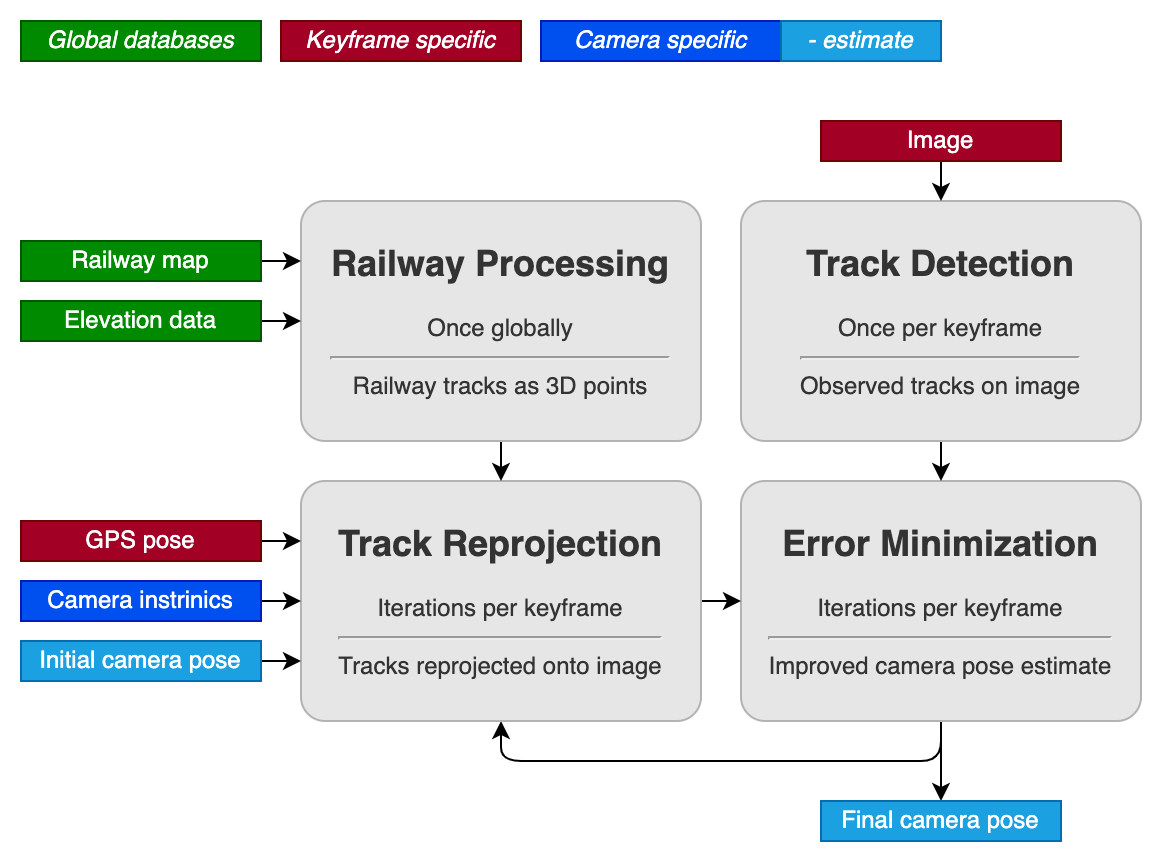
\includegraphics[width=0.9\textwidth]{images/overview}
    \caption{Overview of the components, interactions, and inputs/outputs color-coded by type (green: global map, red: frame-specific, and blue: camera-specific).}
    \label[figure]{fig:method_overview}
\end{figure}


\section{Map Processing}
\label[section]{sec:method_map_processing}

In this component, raw map data is processed into a 3D point cloud for each railway track that is more usable for downstream components, particularly Track Reprojection. The raw map data includes a railway network in the form of an OpenStreetMap (OSM) file (illustrated in \cref{fig:osm_railway_network}), as well as elevation data. The output is a set of 3D points for each railway track.

The process includes extracting the nodes and tracks from the railway map, converting them to 2D splines sorted by tracks, then filling the gaps between the points to achieve more regular spacing, and finally adding elevation data to obtain a 3D point cloud for each track. An overview of the input, process, and output is shown in \cref{tab:map_processing}.

\begin{table}[h]
    \caption{Map processing component: input, process, and output.}
    \begin{tabularx}{\textwidth}{| l | X |}
        \hline
        \textbf{Input:} & \begin{itemize}
            \item Railway network (OSM file)
            \item Elevation data
        \end{itemize} \\
        \hline
        \textbf{Process:} & \begin{enumerate}
            \item Extract nodes and tracks from railway network
            \item Convert nodes to 2D splines per track
            \item Fill track gaps by 2D interpolation
            \item Add elevation data to get 3D points
        \end{enumerate} \\
        \hline
        \textbf{Output:} & \begin{itemize}
          \item Railway tracks as 3D point clouds
        \end{itemize} \\
        \hline
    \end{tabularx}
    \label[table]{tab:map_processing}
\end{table}

Overall, the initial data is enhanced, while also being reduced to what is actually needed for downstream components -- only in the relevant area that is a combined map of all specified frames. Even though processing a combined map of all keyframes takes more time once, it is much faster than processing the railway surrounding each frame location individually, since points may overlap. Moreover, this is the only way to ensure that large railway gaps do not lead to a problem of missing data in the reprojection of any single frame, as would be the case otherwise.

\begin{figure}[h]
    \centering
    \includegraphics[width=0.8\textwidth]{images/railway_map.jpg}
    \caption{Railway network from OpenStreetMap (OSM) file.}
    \label[figure]{fig:osm_railway_network}
\end{figure}


\newpage
\section{Track Reprojection}
\label{sec:method_track_reprojection}

In this component, local 3D railway points are reprojected onto each image, given the GPS pose of the current frame, the camera intrinsics, and camera pose estimate. The output is a set of dense, regularly-spaced 2D points on the image.

This is done by first finding local railway tracks, by searching within a radius of interest around the current frame GPS pose, then increasing the point density using 3D interpolation, transforming these points into the camera frame, filtering the points by angle to the camera (to obtain a more regular spacing in image space), and finally reprojecting these points into the image space. An overview of the input, process, and output is shown in \cref{tab:track_reprojection}.

\begin{table}[h]
    \caption{Track reprojection component: input, process, and output.}
    \begin{tabularx}{\textwidth}{| l | X |}
        \hline
        \textbf{Input:} & \begin{itemize}
            \item Railway tracks as 3D point clouds
            \item GPS pose
            \item Camera pose estimate
            \item Camera intrinsics
        \end{itemize} \\
        \hline
        \textbf{Process:} & \begin{enumerate}
            \item Find local railway tracks -- search radius of interest
            \item Increase point density by 3D interpolation of tracks
            \item Transform points into camera frame
            \item Filter number of points by angle to camera
            \item Reproject onto image
        \end{enumerate} \\
        \hline
        \textbf{Output:} & \begin{itemize}
        \item Reprojected local tracks
        \end{itemize} \\
        \hline
    \end{tabularx}
    \label[table]{tab:track_reprojection}
\end{table}

In contrast to the previous component, this process is run for each frame individually, and the reprojection step is repeated at each iteration of the camera pose, which is iterated over in the Pose Optimization component. This means that the filtered, dense points in 3D space are constant throughout the iterations per frame, yet reprojected differently for each camera pose.

\begin{figure}[h]
    \centering
    \begin{minipage}[t]{0.48\textwidth}
        \includegraphics[width=\textwidth]{images/0570_reprojected.jpg}
    \end{minipage}
    \hfill
    \begin{minipage}[t]{0.48\textwidth}
        \includegraphics[width=\textwidth]{images/5410_reprojected.jpg}
    \end{minipage}
    \caption{Reprojected enhanced railway tracks (red) and original nodes (yellow).}
    \label[figure]{fig:track_reprojection}
\end{figure}


\newpage
\section{Track Detection}
\label{sec:method_track_detection}

In this component, visible railway tracks are observed in each image, currently by manual annotation but expandable to automated detection. The output is a set of dense 2D points for each observed track.

The process consists of manually annotating points along the tracks in each image, converting these points to 2D splines, and increasing the point density by 2D interpolation. An overview of the input, process, and output is shown in \cref{tab:track_detection}, while the annotated points and interpolated output is shown in \cref{fig:track_detection}.

\begin{table}[h]
    \caption{Track detection component: input, process, and output.}
    \begin{tabularx}{\textwidth}{| l | X |}
        \hline
        \textbf{Input:} & \begin{itemize}
            \item Image
        \end{itemize} \\
        \hline
        \textbf{Process:} & \begin{enumerate}
            \item Manually annotate 2D points in images
            \item Convert to 2D splines
            \item Increase point density by 2D interpolation
        \end{enumerate} \\
        \hline
        \textbf{Output:} & \begin{itemize}
        \item Observed tracks as 2D points
        \end{itemize} \\
        \hline
    \end{tabularx}
    \label[table]{tab:track_detection}
\end{table}

This component is not yet implemented with machine learning since the focus of this project was on the optimization algorithm and reprojection pipeline. As such, manual annotation is used to obtain ground truth data for the evaluation of the Pose Optimization component. Nevertheless, track detection is a crucial part of the pipeline, and should be integrated in future work in order to obtain a fully automated and generalizable pipeline.

\begin{figure}[h]
    \centering
    \begin{minipage}[t]{0.48\textwidth}
        \includegraphics[width=\textwidth]{images/0570_annotated.jpg}
    \end{minipage}
    \hfill
    \begin{minipage}[t]{0.48\textwidth}
        \includegraphics[width=\textwidth]{images/5410_annotated.jpg}
    \end{minipage}
    \caption{Annotated points (light blue) and interpolated splines (dark blue).}
    \label[figure]{fig:track_detection}
\end{figure}

\newpage
\section{Pose Optimization}
\label{sec:method_pose_optimization}

In this component, the camera pose is optimized by minimizing the error between the observed tracks and the reprojected local tracks. The output is an updated camera pose estimate.

This is done by using an iterative closest point (ICP) algorithm. At first, one-to-one correspondences are found between the observed and reprojected points from which residuals are computed, equal to the distance between corresponding points. Second, these residuals are added to the optimization problem and it is solved to obtain a new camera pose estimate. This process is repeated until convergence, with new correspondences found at each iteration. An overview of the input, process, and output is shown in \cref{tab:pose_optimization}, while the correspondences are illustrated in \cref{fig:pose_optimization_correspondences}.

\begin{table}[h]
    \caption{Pose optimization component: input, process, and output.}
    \begin{tabularx}{\textwidth}{| l | X |}
        \hline
        \textbf{Input:} & \begin{itemize}
            \item Observed tracks
            \item Reprojected local tracks
        \end{itemize} \\
        \hline
        \textbf{Process:} & \begin{enumerate}
            \item Find one-to-one correspondences for each observed point
            \item Compute residuals
            \item Add to optimization problem
            \item Solve optimization problem
        \end{enumerate} \\
        \hline
        \textbf{Output:} & \begin{itemize}
        \item New camera pose estimate
        \end{itemize} \\
        \hline
    \end{tabularx}
    \label[table]{tab:pose_optimization}
\end{table}

Specifically, one-to-one correspondences are found as follows: for each observed point, the closest reprojected point is found. If a reprojected point happens to be associated to multiple observed points, only the closest observed point remains associated to the reprojected point, while all others are removed and left without correspondence. This is done to ensure that each observed point is associated to only one reprojected point, and vice versa.

\begin{figure}[h]
    \centering
    \begin{minipage}[t]{0.48\textwidth}
        \includegraphics[width=\textwidth]{images/0570_optimization_initial.png}
    \end{minipage}
    \hfill
    \begin{minipage}[t]{0.48\textwidth}
        \includegraphics[width=\textwidth]{images/5410_optimization_initial.png}
    \end{minipage}
    \caption{Initial correspondences (green) between reprojected points (red) and observed points (blue).}
    \label[figure]{fig:pose_optimization_correspondences}
\end{figure}

The optimization problem can be solved as single-frame or multi-frame, where the latter implies that multiple frames are optimized in parallel. More details regarding these approaches are provided below.

\subsection*{Single-frame vs. Multi-frame}

% Single-frame optimization process & diagram explained
% 1. use initial camera pose to reproject 3d points
% 2. find correspondences with observed points
% 3. compute residuals & add to optimization problem
% 4. solve optimization problem
% 5. update camera pose estimate
% 6. repeat until convergence

In the single-frame approach, the optimization problem is solved for an individual frame. At first, the initial camera pose estimate is used to reproject the 3D points onto the image plane. Then, correspondences are found between the reprojected points and the observed points. These are used to compute the residuals and add them to the optimization problem, which is then solved to obtain a new camera pose estimate. This process is repeated until convergence, with new correspondences found at each iteration given the updated camera pose. An overview of the process is shown in \cref{fig:optimization_single-frame}.

\begin{figure}[h]
    \centering
    \includegraphics[height=0.5\textwidth]{images/optimization_single-frame.png}
    \caption{Single-frame optimization process.}
    \label{fig:optimization_single-frame}
\end{figure}

% Multi-frame optimization process & diagram explained
% 1. use initial camera pose to reproject 3d points across multiple frames
% 2. find correspondences with observed points
% 3. compute residuals for each frame & add to combined optimization problem
% 4. solve combined optimization problem
% 5. update camera pose estimate
% 6. repeat until convergence

In the multi-frame approach, the optimization problem is solved for multiple frames in parallel. At first, the initial camera pose estimate is used to reproject the 3D points onto the image plane for each frame. Then, correspondences are found between the reprojected points and the observed points for each frame. These are used to compute the residuals and add them to the same combined optimization problem, which is then solved to obtain a new camera pose estimate. This process is repeated until convergence, with new correspondences found for all frames at each iteration given the updated camera pose. An overview of the process is shown in \cref{fig:optimization_multi-frame}.

\begin{figure}[h]
    \centering
    \includegraphics[height=0.5\textwidth]{images/optimization_multi-frame.png}
    \caption{Multi-frame optimization process.}
    \label{fig:optimization_multi-frame}
\end{figure}